\section{Introduction}

The static analysis of source code is performed for many reasons, such as bug detection, security analysis, quality assurance, and more. Many static analysis tools and algorithms exist to assist in detection tasks on source code. However, the manual production of such tools and algorithms can be quite costly in time and money, and are prone to software bugs and human error. Although static analysis tools can be automatically applied to programs, they mostly rely on mappings from code elements to high level concepts to detect bugs related to software semantics. For example, Flowdroid~\cite{arzt2014flowdroid} relies on SuSi~\cite{rasthofer2014machine} to provide the mapping from source and sink API methods to information types, or \textit{pscout}~\cite{au2012pscout} to provide the mapping from API methods to permissions. 

%TODO: Please find one more example if possible.

In existing techniques, the mapping is typically generated manually or semi-automatically (e.g., SuSi is automatically extended from a manually built training set). Besides the huge manual effort required for constructing such mappings, they also have the following three limitations. First of all, libraries and frameworks are often evolving frequently, so the mappings can go out-of-date quickly. \textit{pscout}'s developers have maintained their mappings since 2012, but its most updated mapping still only supports up to Android 5.1.1, which was released in April 2015 (more than three years from now). Similarly, SuSi only has a version for Android 4.2, which was released in July 2012 (more than six years from now). Second, construction of such mappings is doable only when there exists a common library or framework for certain tasks. For example,  Android SDK is just about the only way to collect information from an Android device (with native code as exceptions). By contrast, a lot of areas have multiple or many libraries (e.g., encryption and authentication libraries, J2EE implementations), making it difficult to pre-construct a mapping for them. Third, such mappings can only handle API methods whose high-level semantics are known before the analysis. However, in many scenarios code analysis needs to know high-level semantics of methods or variables defined by client software developers. For example, a code security checking tool may need to know which variables represent user name and password so that it can check whether they are well protected (e.g., encrypted when stored locally and transmitted through secure connection protocols).  

Therefore, a technique that can construct mapping from code elements to high-level concepts without prior preparation will alleviate the above limitations and significantly enhance usability of code analysis tools in practice. In this paper, we describe a technique to map arbitrary code elements to a set of pre-defined high-level concepts. As a basic solution, we can always measure textual similarity between keyword / phrases representing the concept and the identifiers in the code, and for each keyword $k$ we can retrieve all code elements having a similarity with $k$ above a certain threshold. However, developers may use different identifiers to represent the same concept or even use identifiers that are not meaningful (when good coding style is not enforced). So a simple retrieval technique will have rather low recall. 

The novel intuition behind our approach is that, given a high-level concept, similar to its textual context (i.e., texts surrounding a keywords / phrase representing the concept), its code context (i.e., code elements surrounding a variable / method representing the concept) also contains a relationship between it and its relevant concepts. For example, an assignment $a = b$ indicates that the concept represented by $b$ is a sub-concept of the concept represented by $a$, and an assignment $a = b[i]$ indicates that the concept represented by $b$ is a collection, and its element is a sub-concept of $a$. With all these relations from context, we can gradually narrow down the possible concepts a code element can represent by comparing a concept's textual context with its code context. In our approach, we use Word2Vec~\cite{mikolov2013efficient} and deep learning to represent the code / textual context of a concept, as described in detail in Section~\ref{approach}.


\textbf{Motivation Example.} Figure~\ref{example} presents an example for computation and clustering features. A user input is first checked with PhoneNumberUtils.isGlobalPhoneNumber(), and then processed by PhoneNumberUtils.parse().getCountryCode(). Both API methods are mainly used for processing phone numbers, so with them as computer features, we can predict the user input as a phone number even if it does not have a meaningful identifier. Later, this phone number flows to a field called pNumber in class Profile. From the other fields defined in the class (e.g., address) also indicates that this field may be a phone number as they are all components of contact information. From the defined fields, we can also infer that the field zCode should be zip code.

\begin{figure*}
	\centering
	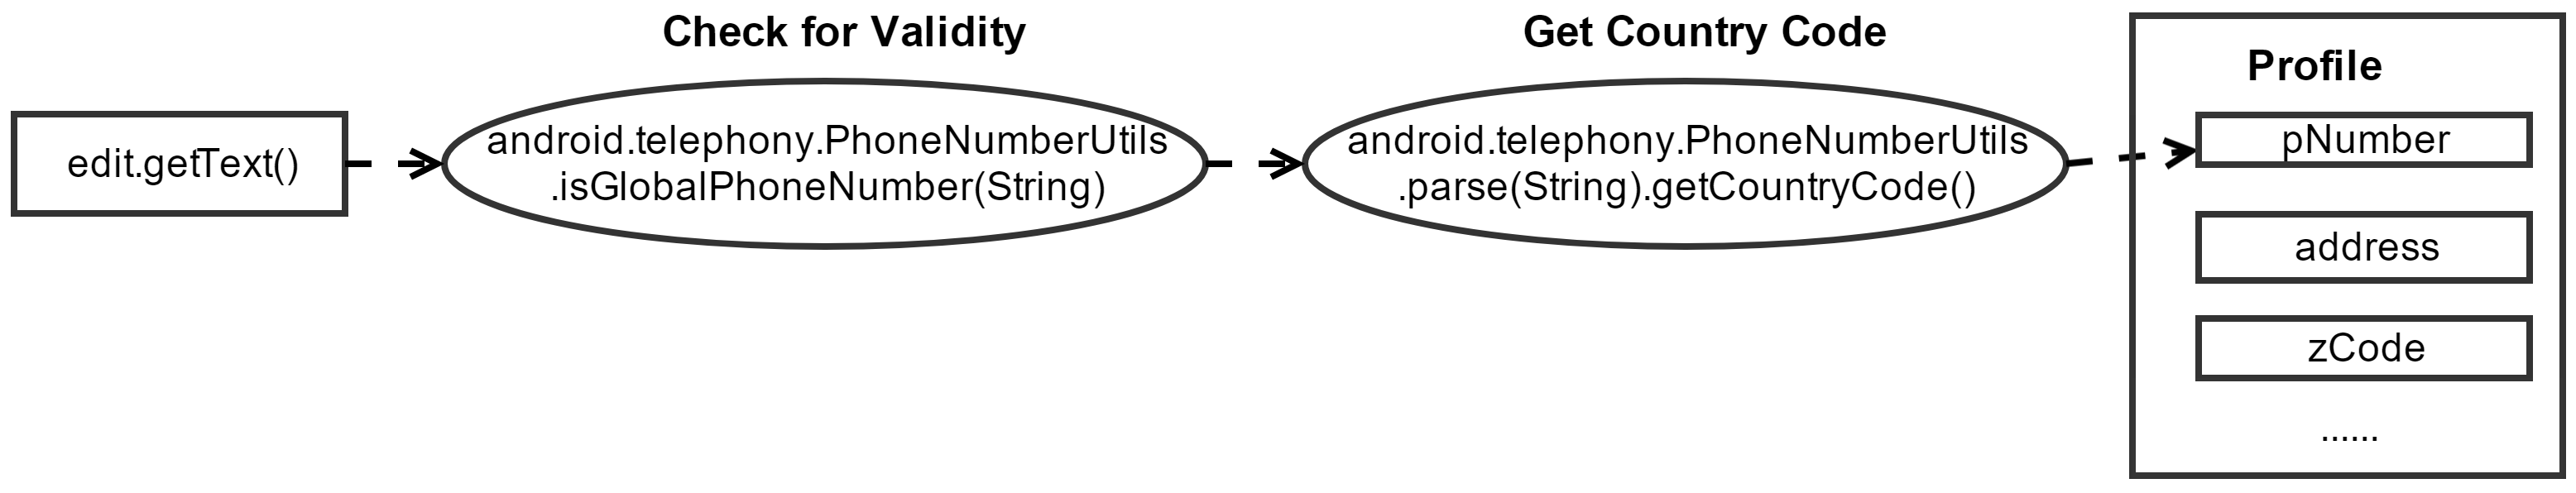
\includegraphics[width=\textwidth]{figures/example_computationOld.png}
	\caption{An Example of Code Context}
	\label{example}
\end{figure*}